\documentclass[12pt]{report}
\usepackage[left=2cm,right=2cm,top=2cm,bottom=2cm]{geometry} % page settings
\usepackage[dutch]{babel} % provides dutch alternatives for english text
\usepackage[utf8]{inputenc} % provides UTF-8 encoding
\usepackage{color} % more color options
\usepackage{enumitem} % options for enumerations
\usepackage{amsmath} % provides many mathematical environments & tools
\usepackage{graphicx} % for displaying images
\usepackage{array}

%DOCUMENT INFORMATION
\title{Samenvatting Statistiek}
\author{Bert De Saffel}
\date{2017-2018}

% CUSTOM COMMANDS
\setlength{\parindent}{0mm}
\setlength{\extrarowheight}{5pt}
\graphicspath{{./img/}}
\newcommand{\todo}[1]{
  {\color{red}\textunderscore{\textit{TODO: #1}}}
}
\newcommand{\exercise}[2]{
  #1
  

  \underline{Oplossing}
  
  #2
  
  \hrulefill
}
\newcommand{\example}[2]{
      \hrulefill
      
      Voorbeeld: #1
      
      #2
      
      \hrulefill
}

\begin{document}
\maketitle
\tableofcontents
 
\part{Herhaling Wiskunde A}
\chapter{Onbepaalde Integralen}
\section{Substitutiemethode}
%Stel $$\alpha = \varphi(t),\;dx = \varphi'(t)$$
%dan $$\int f(\varphi(t))\varphi'(t)dt = \int f(x) dx$$
\subsection{Voorbeeld 1}
\begin{equation*}
	\begin{split}
		\int \frac{t - 1}{t^2 + 4}dt & = \int \frac{t}{t^2 + 4}dt - \int \frac{dt}{t^2 + 4} \\
		\hbox{stel}\;\; &  u = t^2 + 4        \\
		\hbox{dan}\;\; & du = 2tdt \rightarrow dt = \frac{du}{2t} \\
		& \Rightarrow \int \frac{t}{2t u} du - \frac{1}{2}\arctan{\frac{t}{2}} \\
		& = \frac{1}{2}\int \frac{du}{u} - \frac{1}{2}\arctan{\frac{t}{2}}\\
		& = \frac{1}{2}\ln{u} - \frac{1}{2}\arctan{\frac{t}{2}} \\
		& =  \frac{1}{2}\ln{t^2 + 4} - \frac{1}{2}\arctan{\frac{t}{2}} + C
	\end{split}
\end{equation*}
\subsection{Voorbeeld 2}
\begin{equation*}
	\begin{split}
		\int \frac{dy}{e^y + 4e^{-y}} & = \int \frac{e^y}{(e^y)^2 + 4} dy \\
		\hbox{stel}\;\; & u = e^y \\
		\hbox{dan}\;\; & du = e^ydy \rightarrow dy = \frac{du}{e^y}\\
		& \Rightarrow \int \frac{e^y}{e^y(u^2 + 4)} du \\
		& = \int \frac{du}{u^2 + 4} \\
		& = \frac{1}{2}\arctan{\frac{u}{2}}\\
		& = \frac{1}{2}\arctan{\frac{e^y}{2}} + C\\
	\end{split}
\end{equation*}
\section{Partieële integratie}
$$\int u\;dv = uv - \int v\;du$$
\subsection{Voorbeeld 1}
\begin{equation*}
	\begin{split}
		\int \ln(x) dx & = \int 1\cdot \ln(x) dx \\
		\hbox{stel}\; u & = ln(x) \; \hbox{en}\; v = \int dx\\
		\hbox{dan}\; du & = \frac{1}{x}dx \; \hbox{en}\; v = x\\
		& \Rightarrow x\ln(x) - \int x\cdot\frac{1}{x}dx\\
		& = x\ln(x) - \int dx\\
		& = x\ln(x) - x + C
	\end{split}
\end{equation*}
\subsection{Voorbeeld 2}
\begin{equation*}
	\begin{split}
		\int \frac{x + 1}{\cos^2(x)}dx & \\
		\hbox{stel}\; u & = x + 1 \; \hbox{en}\; v = \int \frac{1}{\cos^2(x)}dx\\
		\hbox{dan}\; du & = dx \; \hbox{en}\; v = \tan(x) \\
		& \Rightarrow (x+1)\tan(x) - \int \tan(x)dx  \\
		& = (x+1)\tan(x) + ln|cos(x)| + C  \\
	\end{split}
\end{equation*}
\subsection{Voorbeeld 3}
\begin{equation*}
	\begin{split}
		\int e^{-x}\sin(2x) & \\
		\hbox{stel}\; u & = \sin(2x) \; \hbox{en}\; v = \int e^{-x}dx\\
		\hbox{dan}\; du & = 2\cos(2x)dx \; \hbox{en}\; v = -e^{-x}\\
		& \Rightarrow= -e^{-x}\sin(2x) + 2 \int e^{-x}\cos(2x) dx\\
		\hbox{stel}\; u & = \cos(2x) \; \hbox{en}\; v = \int e^{-x}dx\\
		\hbox{dan}\; du & = -2\sin(2x)dx \; \hbox{en}\; v = -e^{-x}\\
		& \Rightarrow -e^{-x}\sin(2x) + 2\bigg[-e^{-x}\cos(2x)  - 2\int e^{-x}\sin(2x)dx   \bigg]\\
		& = -e^{-x}\sin(2x) - 2e^{-x}\cos(2x) -  4\int e^{-x}\sin(2x)dx\\
	\end{split}
\end{equation*}
Dus
\begin{equation*}
	\begin{split}
		& \int e^{-x}\sin(2x)  = -e^{-x}\sin(2x) - 2e^{-x}\cos(2x) -  4\int e^{-x}\sin(2x)dx \\
		\Leftrightarrow\; &  5\int e^{-x}\sin(2x) = -e^{-x}[\sin(2x) + 2\cos(2x)] \\
		\Leftrightarrow\; & \int e^{-x}\sin(2x) = \frac{-e^{-x}[\sin(2x) + 2\cos(2x)]}{5}
	\end{split}
\end{equation*}
\subsection{voorbeeld 4}
\begin{equation*}
	\begin{split}
		\int \sin^4(\theta) d\theta & = \int (\sin^2(\theta))^2 d\theta \\
		& = \int \bigg(\frac{1 - \cos(2\theta)}{2}\bigg)^2 d\theta \\
		& = \int \bigg(\frac{1}{4} - \frac{\cos(2\theta)}{2} + \frac{\cos^2(2\theta)}{4} \bigg)d\theta \\
		& = \int \frac{1}{4}d\theta - \int \frac{\cos(2\theta)}{2}d\theta + \int \frac{\cos^2(2\theta)}{4}d\theta \\
		& = \frac{\theta}{4} - \frac{\sin(2\theta)}{4} + \frac{\sin(4\theta) + 4\theta}{32} \\
		& = \frac{12\theta - 8\sin(2\theta) + \sin(4\theta)}{32} + C
	\end{split}
\end{equation*}
\part{Wiskunde B}
\chapter{Differentiaalvergelijking}
\section{Definities}
De algemene definitie is:
$$F(x, y, y', y'', ..., y^{(n)}) = 0$$
waarbij: \begin{itemize}
\item \textbf{x} een veranderlijke is.
\item \textbf{y} een functie van x is.
\item er minstens één afgeleide van y is.
\end{itemize}
\example{Differentiaalvergelijking}{
	$$ x + y + y' = 0$$
}

Een differentiaalvergelijking heeft een \textbf{orde} en een \textbf{graad}
\begin{itemize}
	\item \textbf{Orde}: Dit is de orde van de hoogste afgeleide dat voorkomt, dus \textit{n}.
	\item \textbf{Graad}: De graad \textit{r} bestaat niet altijd maar is wel altijd een strik positief geheel getal. De graad is de macht die behoort tot de afgeleide met de grootste orde. $y^{(n)^{r}}$
\end{itemize}
\example{Orde en graad}{
	\begin{center}
		\begin{tabular}{l | l | l}
			Differentiaalvergelijking                          & Orde & Graad \\
			\hline
			$y\ - 2y'^3 = yx$                                  & 2    & 1     \\
			$1 + (y'')^4 + 2y' + x(y''')^2 = sin(x)$           & 3    & 2     \\
			$(x - 1)(y'') - xy' + y = 0$                       & 2    & 1     \\
			$e^s\frac{d^3s}{dt^3} + (\frac{ds^2}{dt^2})^3 = 0$ & 3    & 1     \\
			$xy' + e^{y'} + y'' = 1$                           & 1    & /     \\
			\hline
			$\sin\sqrt {y'} = x + 2$                           & 1    & /     \\
			$\;\;\rightarrow y' = \arcsin^2(x+2)$              & 1    & 1     \\
			\hline
			$\sin y' = xy'^2$                                  & 1    & /     \\
			$\;\;\rightarrow y' = \arcsin(xy'^2)$              & 1    & /     \\
			\hline
			$y^{'3} + \frac{x}{y''} + y'' = 1$                 & 2    & ?     \\
			$\;\;\rightarrow y^{'3}y'' + x + (y'')^2 = 1$      & 2    & 2     
			   
		\end{tabular}
	\end{center}
}
\section{Soorten oplossingen}
Tijdens het oplossen van een differentiaalvergelijking van de \textit{n}-de orde worden drie oplossingen onderscheden:
\begin{enumerate}
 \item De \textbf{Algemene oplossing (AO)}: Verzameling van functies zodat de differentiaalvergelijking klopt. De algemene oplossing bevat \textit{n }onafhankelijke constanten. Deze constanten zijn getallen en geen functies.
 \item De \textbf{Particuliere oplossing (PO)}: Dit is één van de krommen van de AO en is afhankelijk van de beginvoorwaarden van het probleem.
 \item De \textbf{Singuliere oplossing (SO)}: Een oplossing die niet voldoet aan de AO maar wel een oplossing is voor de DVG.
\end{enumerate}
\example{Onafhankelijke variabelen:}
{
  \begin{center}
    \begin{tabular}{l | l | l}
      AO & Onafh. C & Orde DVG \\
      \hline
      $y = C_1 + C_2x$ & 2 & 2 \\
      $y = C_1  - C_1^2x$ & 1 & 1 \\
      \hline
      $y = C_1(C_2 + C_3e^x)$ & ? & ? \\
      $\;\;\rightarrow C_1C_2 + C_1C_3e^x$ & ? & ? \\
      $\;\;\rightarrow a + be^x$ & 2 & 2 \\
      \hline
      $y = C_1 + \ln(C_2 x)$ & ? & ? \\
      $\;\;\rightarrow y = C_1 + \ln(C_2) + \ln(x)$ & ? & ? \\
      $\;\;\rightarrow y = a + \ln(x)$ & 1 & 1

   
    \end{tabular}
  \end{center}
}
\example{Oef 1 AO en PO}{Gegeven een differentiaalvergelijking: $y'' + y = 0$
\begin{enumerate}
 \item Toon aan dat $y = a\sin(x) + b\cos(x)$ de AO is.
 \item Geef enkele PO's.
 \end{enumerate}
Oplossing:
\begin{enumerate}
 \item 
  \begin{equation*}
   \begin{split}
    y & = a\sin(x) + b\cos(x) \\
    y' & = a\cos(x) - b\sin(x) \\
    y'' & = -a\sin(x) - b\cos(x) 
   \end{split}
  \end{equation*}
  Hieruit volgt:
  \begin{gather*}
    y'' + y  = 0 \\
    -a\sin(x) - b\cos(x) + \sin(x) + b\cos(x)  = 0  \\
    \rightarrow \hbox{Het is een oplossing}
  \end{gather*}
  De differentiaalvergelijking heeft orde 2. De y-vergelijking bevat 2 onafhankelijke constanten en de y-vergelijking is een oplossing. Hierdoor is y de AO van de differentiaalvergelijking.
 \item Enkele PO's:
 \begin{equation*}
 \begin{split}
  y & = 0\\
  y & = \sqrt{2}\sin(x) \\
  y & = \sin(x) + \cos(x)
 \end{split}
 \end{equation*}
\end{enumerate}
}

\example{Oef 2 AO en PO}
{Gegeven een differentiaalvergelijking: $y'^2 - yy'+e^x$
\begin{enumerate}
 \item Geef de orde en graad.
 \item Is $y = \frac{1}{C} + Ce^x$ de AO?
 \item Wat  voor soort oplossing is $y = 2\sqrt{e^x}$
 \end{enumerate}
Oplossing:
\begin{enumerate}
 \item 
   De orde is 1 en de graad is 2.
 
 \item 
 $$y' = Ce^x$$
 \begin{equation*}
  \begin{split}
   \rightarrow C^2(e^x)^2 - (\frac{1}{C} + Ce^x)Ce^x + e^x &  = 0 \\
   \Leftrightarrow C^2e^{2x} - e^x - C^2e^{2x} + e^x &  = 0 \\
   \Leftrightarrow C^2e^{2x} - e^x - C^2e^{2x} + e^x & = 0 \\
   \Leftrightarrow 0 & =0
  \end{split}
 \end{equation*}
  $$\rightarrow \hbox{Het is een oplossing}$$
  Orde DVG = 1 = Onafhankelijke constanten van y
 
 \item 
 $$ y'  = 2 \cdot \frac{1}{2\sqrt{e^x}} \cdot e^x = \sqrt{e^x}$$
 \begin{equation*}
  \begin{split}
   \rightarrow & y'^2 - yy'+e^x \\
   \Leftrightarrow &  (\sqrt{e^x})^2 - 2\sqrt{e^x}\cdot\sqrt{e^x} + e^x  = 0 \\
   \Leftrightarrow & e^x - 2e^x + e^x  = 0 \\
   \Leftrightarrow & 0 = 0
  \end{split}
 \end{equation*}
  Dit is een singuliere oplossing aangezien y niet overeenkomt met de AO, maar wel voldoet aan de DVG.
 
\end{enumerate}
}
\section{Bepalen van een DVG}
Indien een AO gegeven is met \textit{n} onafhankelijke constanten:
\begin{enumerate}
 \item Controleer of de constanten werkelijk onafhankelijk zijn.
 \item Leid de AO \textit{n} maal af.
 \item Elimineer de \textit{n} constanten van de \textit{n + 1} bekomen vergelijkingen. De laatste vergelijking moet zeker gebruikt worden.
 \item Controleer of de DVG van orde \textit{n} is.
\end{enumerate}

\example{Oef 1 bepalen van een DVG}
{
  De algemene oplossing is $$y = C_1 + C_2x$$
  \begin{enumerate}
   \item Er zijn \textit{2} onafhankelijke constanten.
   \item Er moet \textit{2} keer afgeleid worden:
   $$
      \begin{cases}
	y    & = C_1 + C_2x \\
	y'   & = C_2 \\
	y''  & = 0 \\
      \end{cases}
   $$
   \item De constanten zijn al geëlimineerd. 
   \item De DVG is $y'' = 0$ en heeft orde \textit{2}.

  \end{enumerate}
}

\example{Oef 2 bepalen van een DVG}
{
  Bepaal de DVG van: $$y = C_1 + C_2e^{-x} + C_3e^{3x}$$
  \begin{enumerate}
   \item Er zijn \textit{3} onafhankelijke constanten.
   \item Er moet \textit{3} maal afgeleid worden.
    \[ 
      \begin{cases}
			y & = C_1 + C_2e^{-x} + C_3e^{3x} \\
	y'     & = -C_2e^{-x} + 3C_3e^{3x}     \\
	y'' & = C_2e^{-x} + 9C_3e^{3x}      \\
	y''' & = -C_2e^{-x} + 27C_3e^{3x}
      \end{cases}
    \]

  \item 
  Tel de 1ste afgeleide op met de 2de afgeleide en tel de 2de afgeleide op met de 3rde afgeleide
  \[
    \begin{cases}
      y + y''    & = 3C_3e^{3x} + 9C_3e^{3x} = 12C_3e^{3x}  \\
      y'' + y''' & = 9C_3e^{3x} + 27C_3e^{3x} = 36C_3e^{3x}
    \end{cases}
  \]
  Vermenigvuldig de 1ste vergelijking met 3 en trek hiervan de 2de vergelijking af.
  
  $$3(y + y'') - y'' - y''' = 3(12C_3e^{3x}) - 36C_3e^{3x} = 0$$
  $$\rightarrow y''' - 2y'' - 3y' = 0$$
  \item
  De orde van deze DVG is \textit{3}
   
  \end{enumerate}
}

\example{Oef 3 bepalen van een DVG}
{
  Bepaal de DVG van alle cirkels met middelpunt y = -x.
  \begin{enumerate}
   \item Eerst moet de AO gevonden worden. Het middelpunt van elke cirkel kan gegeven worden met $m(a, -a).$
    Hieruit volgt de algemene vergelijking van een cirkel: $$(x - a)^2 + (y + a)^2 = R^2$$
    Er zijn \textit{2} onafhankelijke constanten (a en R).
   \item Er moet \textit{2} maal (impliciet) afgeleid worden.
   \[
      \begin{cases}
       (x - a)^2 + (y + a)^2 = R^2 \\
       \frac{dy}{dx} : (x-a) + y'(y+a) = 0 \\
       \frac{d^2y}{dx^2} : 1 + y''(y + a) + y'^2 = 0
      \end{cases}
   \]
   \item
    Vorm $\frac{dy}{dx}$ om naar $a$:
    $$a = \frac{-x - yy'}{y' - 1}$$
    Substitueer deze $a$ in $\frac{d^2y}{dx^2}$:
    $$1 + y''(y + (\frac{-x - yy'}{y' - 1})) + y'^2 = 0$$
    $$\rightarrow 1 + y''(y + (\frac{x + yy'}{-y' + 1})) + y'^2 = 0$$
    $$\rightarrow y''(x + y) - y'^3 + y'^2 - y' + 1 = 0$$
   \item Orde van de DVG = \textit{2}  = Aantal onafhankelijke constanten.
  \end{enumerate}
}


\chapter{Laplacetransformatie}
\section{De Heaviside functie}
De Heaviside functie heeft als voorschrift:
$$H(t - \alpha) = 
\begin{cases}
  0 \;\; t < \alpha \\
  1 \;\; t > \alpha
\end{cases}$$

\example{Voorbeeld Heaviside functie}
{
Teken over $x=[-3,4]$ de functie $y = 2H(t + 2) - tH(t) + (t+t^2)H(t-2)$.

Er zijn veranderingen bij $t = -2, t = 0$ en $t = 2$.

    \begin{tabular}{l | l}
    \hline
    $2\cdot(0) - t\cdot(0) + (t+t^2)\cdot(0) = 0$ & $t < -2$\\
    $2\cdot(1) - t\cdot(0) + (t+t^2)\cdot(0) = 2$ & $-2 < t < 0$  \\
    $2\cdot(1) - t\cdot(1) + (t+t^2)\cdot(0) = 2 - t$ & $0 < t < 2$\\
    $2\cdot(1) - t\cdot(1) + (t+t^2)\cdot(1) = 2 + t^2$ & $t > 2$\\
    \end{tabular}
  \todo{graph}
}

\part{Oefeningen}
\chapter{Differentiaalvergelijkingen}
\exercise{Bepaal de DVG van \begin{enumerate}
                          \item $y = C_1x + C_2$
                          \item de cirkels met hun middelpunt op de x-as 
                          \item de raaklijnen aan $K: y = x^2$
                         \end{enumerate}}
{
\begin{enumerate}
 \item De vergelijking $y = C_1x + C_2$ heeft 2 onafhankelijke constanten. Er moet dus 2 keer afgeleid worden.
 \begin{equation*}
  \begin{split}
   y' & = C_1 \\
   y'' & = 0
  \end{split}
 \end{equation*}
 De differentiaalvergelijking is $y'' = 0$
 \item Het middelpunt op de x-as kan gedefinieerd worden als $m \in x-as \Rightarrow m(C_1, 0)$. De straal wordt gedefinieerd als $C_2$. De vergelijking van een cirkel wordt dan:
 $$\Gamma: (x - C_1)^2 + y^2 = C_2^2$$
 Er zijn 2 onafhankelijke constanten. Er moet dus 2 keer (impliciet) afgeleid worden.
 \begin{equation*}
  \begin{split}
   \frac{dy}{dx} :\; & 2(x - C_1) + 2yy' = 0 \\
   \frac{d^2y}{dx^2} :\; & 2 + 2(y'y' + yy'') = 0
  \end{split}
 \end{equation*}
 De 2de afgeleide bevat geen constanten meer dus de differentiaalvergelijking wordt: 
 $$yy'' + (y')^2 + 1 = 0$$
 \item De raaklijn wordt gegeven door : $R: y - y'p = y'_p(x - x_p)$
 
 Stel $p \in K$ en $x_p = C$:
 \begin{equation*}
  \begin{split}
   \Rightarrow & y_p = (x_p)^2 = C^2 \\
   \Rightarrow & p(C, C^2)
  \end{split}
 \end{equation*}
  De richtingscoëfficient $y'_p$ wordt gegeven door 
  $$y'= 2x \Rightarrow y'_p = 2C$$
  
  De formule van de raaklijn kan worden ingevuld:
  $$R: (y - C^2) = 2C(x - C)$$
  Deze vergelijking bevat slechts 1 constante en moet dus 1 maal afgeleid worden.
  $$y' = 2C \Leftrightarrow C = \frac{y'}{2}$$
  Substitueer $C$ in de formule van de raaklijn:
  \begin{equation*}
   \begin{split}
    & y - \bigg(\frac{y'}{2}\bigg)^2 = y'\bigg(\frac{y'}{2}\bigg)\bigg(x - \frac{y'}{2}\bigg) \\
    \Leftrightarrow \; & 4y - y'^2 = 4xy' - 2y'^2 \\
    \Leftrightarrow \; & y'^2 - 4y'x + 4y = 0
   \end{split}
  \end{equation*}
  is de differentiaalvergelijking.
\end{enumerate}
}

\chapter{Laplacetransformatie}
\section{De Heaviside functie}
\exercise{Gegeven 
$$f(t) = \begin{cases}
          0 & t < = 0 \\
          t & 0 < t < 1 \\
          2 - t & 1 < t < 2 \\
          0 & t > 2
         \end{cases}
$$ 
en
$$g(t) = \begin{cases}
          0 & t < 0 \\
          1 & 0 < t < 3 \\
          e^tt^2 & t > 3
         \end{cases}
$$
Druk $f(t)$ en $g(t)$ uit a.d.h.v. de Heaviside-functie.}{
\begin{equation*}
 \begin{split}
  f(t) & = H(t- 0)(-0 + t) + H(t - 1)(-t + 2 -t) + H(t - 2)(-2(2-t) + 0) \\
       & = H(t)t + H(t-1)(2-2t) + H(t-2)(t-2)
 \end{split}
\end{equation*}
\begin{equation*}
 \begin{split}
  g(t) & = H(t - 0)(-0 + 1) + H(t - 3)(-1 + e^tt^2)
 \end{split}
\end{equation*}
}

\exercise{Gegeven $$g(t) = \begin{cases}
                            0 & t < 0 \\
                            t &  0 < t < \frac{\pi}{2} \\
                            \sin t & \frac{\pi}{2} < t < \pi \\
                            0 & t > \pi         
                           \end{cases}
$$
Druk $g(t)$ uit a.d.h.v. de Heaviside functie en maak een tekening.}{
\begin{equation*}
 \begin{split}
  g(t) & = H(t)(-0 + t) + H(t - \frac{\pi}{2})(-t + \sin t) + H(t - \pi)(-\sin t + 0) \\
       & = H(t)t + H(t - \frac{\pi}{2})(\sin t - t) + H(t - \pi)(-\sin t) \\
       & = H(t)t + H(t - \frac{\pi}{2})(\sin t - t) - H(t - \pi)\sin t
 \end{split}
\end{equation*}
\begin{center}
 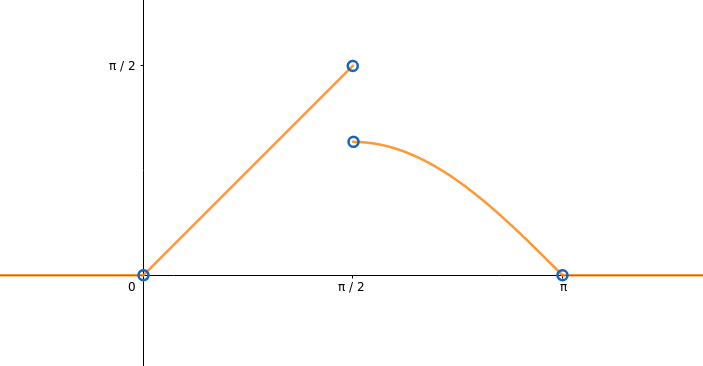
\includegraphics[width=\textwidth]{oef2_heaviside}
\end{center}
}

\exercise{Gegeven de grafiek van de functie $h(t)$. Bepaal het voorschrift van $h(t)$ en druk uit a.d.h.v. de Heaviside functie.
\begin{center}
 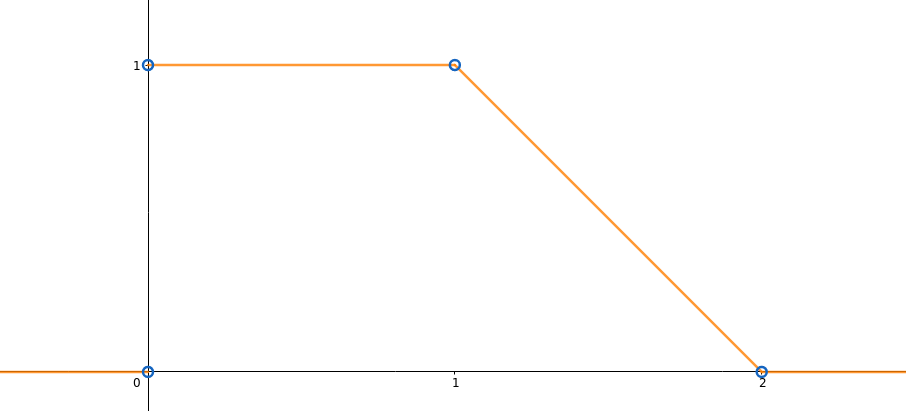
\includegraphics[width=\textwidth]{oef3_heaviside}
\end{center}}{
De functie kan geschreven worden als:
$$h(t) = \begin{cases}
          0 & t < 0 \\
          1 & 0 < t < 1 \\
          2 - t & 1 < t < 2 \\
          0 & t > 2
         \end{cases}
$$
Hieruit volgt gemakkelijk de Heaviside versie hiervan:
\begin{equation*}
 \begin{split}
  h(t) & = H(t)(-0 + 1) + H(t - 1)(-1 + (2 - t)) + H(t-2)(-(2-t) + 0) \\
       & = H(t) + H(t-1)(1 - t) + H(t- 2)(t - 2)
 \end{split}
\end{equation*}


}
         
\end{document}

